\documentclass{article}

\usepackage{amsmath,amssymb}
\usepackage{tikz}
\usepackage{xcolor}
\usepackage[left=2.1cm,right=3.1cm,bottom=3cm,footskip=0.75cm,headsep=0.5cm]{geometry}
\usepackage{enumerate}
\usepackage{enumitem}
\usepackage{marvosym}

\usepackage[utf8]{inputenc}

\renewcommand*{\arraystretch}{1.4}

\title{\textbf{Einführung in die Informatik, Übung 8}}
\author{\textsc{Henry Haustein}}
\date{}

\begin{document}
	\maketitle
	
	\section*{Aufgabe 8.1}
	
	\begin{enumerate}[label=(\alph*)]
		\item $2^Q=\mathcal{P}(Q)=\{\emptyset,\{q_0\},\{q_1\},\{q_2\},\{q_0,q_1\},\{q_0,q_2\},\{q_1,q_2\},\{q_0,q_1,q_2\}\}$, $F'=\{\{q_1\},\{q_0,q_1\},\{q_1,q_2\},\{q_0,q_1,q_2\}\}$ $\Rightarrow$ $\mathcal{A}'=(2^Q,\Sigma,\{q_0\},\delta,F')$ mit $\delta$
		\begin{center}
			\begin{tikzpicture}[scale=0.95]
			\node[circle,draw=black, fill=white] (q0) at (-6,0) {$\{q_0\}$};
			\node[circle,draw=black, fill=white,double] (q1) at (0,2) {$\{q_1\}$};
			\node[circle,draw=black, fill=white] (q2) at (3,2) {$\{q_2\}$};
			\node[circle,draw=black, fill=white,double] (q0q1) at (-3,0) {$\{q_0,q_1\}$};
			\node[circle,draw=black, fill=white] (q0q2) at (0,-2) {$\{q_0,q_2\}$};
			\node[circle,draw=black, fill=white,double] (q1q2) at (6,0) {$\{q_1,q_2\}$};
			\node[circle,draw=black, fill=white,double] (q0q1q2) at (0,-6) {$\{q_0,q_1,q_2\}$};
			\node[circle,draw=black, fill=white] (e) at (0,6) {$\emptyset$};
			
			\draw[->] (-7,0) -- (q0);
			\draw[->] (q0) to[bend left=30] node[midway,above] {$a$} (q0q1);
			\draw[->] (q0q1) to[bend left=30] node[midway,below] {$c$} (q0);
			\draw[->] (q0) to node[midway,above left] {$b$} (e);
			\draw[->] (q0q1q2) to[bend left=20] node[midway,above right] {$c$} (q0);
			\draw[->] (q0q1) to node[midway,below left] {$b$} (q0q2);
			\draw[->] (q0q2) to[bend left=30] node[midway,below] {$c$} (q0);
			\draw[->] (q0q2) to[bend left=30] node[midway,left] {$b$} (q1);
			\draw[->] (q1) to[bend left=30] node[midway,right] {$b$} (q0q2);
			\draw[->] (q0q2) to node[midway,left] {$a$} (q0q1q2);
			\draw[->] (q1) to node[midway,left] {$a,c$} (e);
			\draw[->] (q2) to node[midway,above] {$b$} (q1);
			\draw[->] (q1q2) to node[midway,above right] {$a$} (q2);
			\draw[->] (q1q2) to node[midway,above left] {$b$} (q0q1q2);
			\draw[->] (q1q2) to[bend right=10] node[midway,above right] {$c$} (e);
			\draw[->] (q2) to node[midway,below left] {$c$} (e);
			\draw[->,looseness=4] (q0) to[out=60,in=120] node[midway,above] {$c$} (q0);
			\draw[->,looseness=4] (q0q1) to[out=60,in=120] node[midway,above] {$a$} (q0q1);
			\draw[->,looseness=4] (q2) to[out=-60,in=-120] node[midway,below] {$a$} (q2);
			\draw[->,looseness=4] (q0q1q2) to[out=-60,in=-120] node[midway,below] {$a,b$} (q0q1q2);
			\draw[->,looseness=4] (e) to[out=60,in=120] node[midway,above] {$a,b,c$} (e);
			\end{tikzpicture}
		\end{center}
		\item Den Automaten, der die Sprache $L(\mathcal{A})$ akzeptiert, konstruiert man, indem man den zugehörigen DEA konstruiert (Aufgabe (a)) und die Endzustände anpasst: $F=Q\setminus F$
		\begin{center}
			\begin{tikzpicture}[scale=0.95]
			\node[circle,draw=black, fill=white,double] (q0) at (-6,0) {$\{q_0\}$};
			\node[circle,draw=black, fill=white] (q1) at (0,2) {$\{q_1\}$};
			\node[circle,draw=black, fill=white,double] (q2) at (3,2) {$\{q_2\}$};
			\node[circle,draw=black, fill=white] (q0q1) at (-3,0) {$\{q_0,q_1\}$};
			\node[circle,draw=black, fill=white,double] (q0q2) at (0,-2) {$\{q_0,q_2\}$};
			\node[circle,draw=black, fill=white] (q1q2) at (6,0) {$\{q_1,q_2\}$};
			\node[circle,draw=black, fill=white] (q0q1q2) at (0,-6) {$\{q_0,q_1,q_2\}$};
			\node[circle,draw=black, fill=white] (e) at (0,6) {$\emptyset$};
			
			\draw[->] (-7,0) -- (q0);
			\draw[->] (q0) to[bend left=30] node[midway,above] {$a$} (q0q1);
			\draw[->] (q0q1) to[bend left=30] node[midway,below] {$c$} (q0);
			\draw[->] (q0) to node[midway,above left] {$b$} (e);
			\draw[->] (q0q1q2) to[bend left=20] node[midway,above right] {$c$} (q0);
			\draw[->] (q0q1) to node[midway,below left] {$b$} (q0q2);
			\draw[->] (q0q2) to[bend left=30] node[midway,below] {$c$} (q0);
			\draw[->] (q0q2) to[bend left=30] node[midway,left] {$b$} (q1);
			\draw[->] (q1) to[bend left=30] node[midway,right] {$b$} (q0q2);
			\draw[->] (q0q2) to node[midway,left] {$a$} (q0q1q2);
			\draw[->] (q1) to node[midway,left] {$a,c$} (e);
			\draw[->] (q2) to node[midway,above] {$b$} (q1);
			\draw[->] (q1q2) to node[midway,above right] {$a$} (q2);
			\draw[->] (q1q2) to node[midway,above left] {$b$} (q0q1q2);
			\draw[->] (q1q2) to[bend right=10] node[midway,above right] {$c$} (e);
			\draw[->] (q2) to node[midway,below left] {$c$} (e);
			\draw[->,looseness=4] (q0) to[out=60,in=120] node[midway,above] {$c$} (q0);
			\draw[->,looseness=4] (q0q1) to[out=60,in=120] node[midway,above] {$a$} (q0q1);
			\draw[->,looseness=4] (q2) to[out=-60,in=-120] node[midway,below] {$a$} (q2);
			\draw[->,looseness=4] (q0q1q2) to[out=-60,in=-120] node[midway,below] {$a,b$} (q0q1q2);
			\draw[->,looseness=4] (e) to[out=60,in=120] node[midway,above] {$a,b,c$} (e);
			\end{tikzpicture}
		\end{center}
	\end{enumerate}
	
	\section*{Aufgabe 8.2}
	
	\begin{enumerate}[label=(\alph*)]
		\item ist erkennbar, der zugehörige Automat ist $\mathcal{A}=(\{q_0,...,q_5\},\{a,b\},q_0,\Delta_a,\{q_5\})$ mit $\Delta_a$
		\begin{center}
			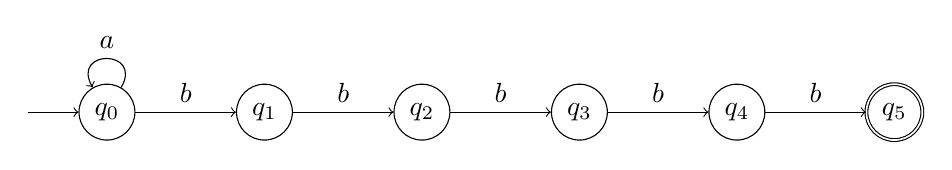
\begin{tikzpicture}
			\node[circle,draw=black, fill=white] (q0) at (0,0) {$q_0$};
			\node[circle,draw=black, fill=white] (q1) at (2,0) {$q_1$};
			\node[circle,draw=black, fill=white] (q2) at (4,0) {$q_2$};
			\node[circle,draw=black, fill=white] (q3) at (6,0) {$q_3$};
			\node[circle,draw=black, fill=white] (q4) at (8,0) {$q_4$};
			\node[circle,draw=black, fill=white,double] (q5) at (10,0) {$q_5$};
			
			\draw[->] (-1,0) -- (q0);
			\draw[->] (q0) to node[midway,above] {$b$} (q1);
			\draw[->] (q1) to node[midway,above] {$b$} (q2);
			\draw[->] (q2) to node[midway,above] {$b$} (q3);
			\draw[->] (q3) to node[midway,above] {$b$} (q4);
			\draw[->] (q4) to node[midway,above] {$b$} (q5);
			\draw[->,looseness=4] (q0) to[out=60,in=120] node[midway,above] {$a$} (q0);
			\end{tikzpicture}
		\end{center}
		\item ist erkennbar, der zugehörige Automat ist $\mathcal{B}=(\{q_0,q_1,q_2,q_3\},\{a\},q_0,\Delta_b,\{q_3\})$ mit $\Delta_b$
		\begin{center}
			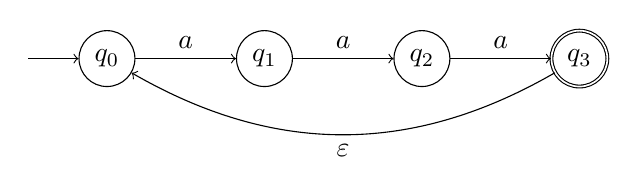
\begin{tikzpicture}
			\node[circle,draw=black, fill=white] (q0) at (0,0) {$q_0$};
			\node[circle,draw=black, fill=white] (q1) at (2,0) {$q_1$};
			\node[circle,draw=black, fill=white] (q2) at (4,0) {$q_2$};
			\node[circle,draw=black, fill=white,double] (q3) at (6,0) {$q_3$};
			
			\draw[->] (-1,0) -- (q0);
			\draw[->] (q0) to node[midway,above] {$a$} (q1);
			\draw[->] (q1) to node[midway,above] {$a$} (q2);
			\draw[->] (q2) to node[midway,above] {$a$} (q3);
			\draw[->] (q3) to[bend left=30] node[midway,below] {$\varepsilon$} (q0);
			\end{tikzpicture}
		\end{center}
		\item ist nicht erkennbar. Angenommen es gäbe einen NEA, der $L_3$ erkennt. Vertauscht man in diesem $a\leftrightarrow b$, so erhält man einen NEA, der $\{a^nb^n\mid n\ge 0\}$ akzeptiert. Da aber $\{a^nb^n\mid n\ge 0\}$ nicht erkennbar ist, kann es dieses Automaten auch nicht geben $\Rightarrow$ \Lightning
		\item vom Gefühl her würde ich sagen, dass diese Sprache nicht erkennbar ist
	\end{enumerate}

	\section*{Aufgabe 8.3}
	
	\begin{enumerate}[label=(\alph*)]
		\item nein, denn es ist nicht möglich ein einzelnes $a$ zu erzeugen \\
		ja, denn
		\begin{center}
			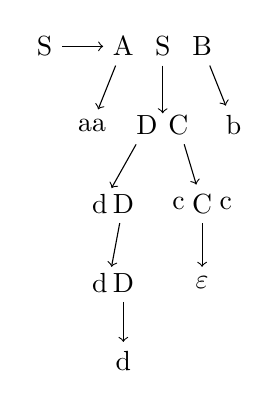
\begin{tikzpicture}
			\node at (0,0) (0) {S};
			\node at (1,0) (1) {A};
			\node at (1.5,0) (2) {S};
			\node at (2,0) (3) {B};
			\node at (0.6,-1) (4) {aa};
			\node at (1.3,-1) (5) {D};
			\node at (1.7,-1) (6) {C};
			\node at (2.4,-1) (7) {b};
			\node at (0.7,-2) (8) {d};
			\node at (1,-2) (9) {D};
			\node at (1.7,-2) (10) {c};
			\node at (2,-2) (11) {C};
			\node at (2.3,-2) (12) {c};
			\node at (0.7,-3) (13) {d};
			\node at (1,-3) (14) {D};
			\node at (2,-3) (15) {$\varepsilon$};
			\node at (1,-4) (16) {d};
			
			\draw[->] (0) -- (1);
			\draw[->] (1) -- (4);
			\draw[->] (2) -- (1.5,-0.85);
			\draw[->] (3) -- (7);
			\draw[->] (5) -- (0.85,-1.8);
			\draw[->] (6) -- (11);
			\draw[->] (9) -- (0.85,-2.8);
			\draw[->] (11) -- (15);
			\draw[->] (14) -- (16);
			\end{tikzpicture}
		\end{center}
		nein, $c$'s lassen sich nicht erzeugen, ohne $d$'s mit zu erzeugen
		\item $L(G)=\{a^{2n}d^mc^kb^n\mid n,m\ge 1,k\ge 0\}$
	\end{enumerate}

	\section*{Aufgabe 8.4}
	
	\begin{enumerate}[label=(\alph*)]
		\item $G=(\{S,A,B\},\{a,b\},P_a,S)$ mit $P_a=\{S\to AB, A\to a, B\to bb, S\to\epsilon\}$
		\item $G=(\{S,A,B\},\{a,b\},P_b,S)$ mit $P_b=\{S\to aSb,S\to A,S\to B,A\to Aa,A\to a,B\to Bb,B\to b\}$
		\item $G=(\{S,A,B,C,D\},\{a,b,c\},P_c,S)$ mit $P_c=\{S\to ABDCA,D\to BDC,D\to A,A\to\varepsilon,A\to aA,B\to b,C\to c\}$
	\end{enumerate}

\end{document}